\documentclass{beamer}
\usepackage[british]{babel}
\usepackage[utf8]{inputenc}
\usepackage{styles/jyumacros}
\usepackage[version=4]{mhchem}
\usepackage{textgreek}
\usefolder{styles}
\usetheme{jyu}

%change these to your own logos if needed (try and match sizes, otherwise, change sizes in Outer Theme file).
\titlegraphic{assets/coverlogo.pdf} %logo on the cover page
\newcommand{\smalllogo}{assets/small_white.pdf} %small logo on frames

%Personal info---------------------------------------------
\title{The MARA-LEB RFQ Guide System}
\date{}
\author[auth]{Jorge Romero}
\institute[inst]{Jyväskylän Yliopisto}
%----------------------------------------------------------

\begin{document}
\begin{frame}
\titlepage
\end{frame}

\begin{frame}{Motivation}
    \vspace*{4em}
    \begin{itemize}
        \item Studying the N=Z region of the nuclear chart 
        \begin{itemize}
            \item<2-> Test predictions of the nuclear shell model
            \item<3-> Increase understanding in the astrophysical rp process
        \end{itemize}
    \end{itemize}
    \vspace*{1em}
   
   \onslide<4->{ MARA-LEB will provide the required efficiency and
    
    selectivity to MARA, a high mass-resolving power
    
    separator in Jyväskylä's Accelerator Lab.}
    \flushright
    \vspace*{-5em}
    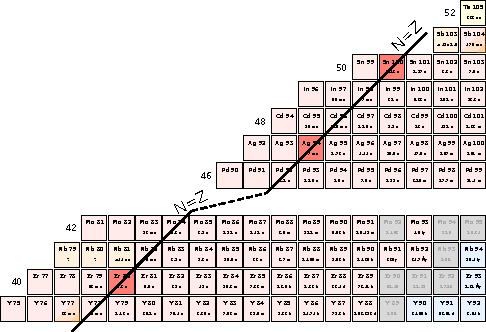
\includegraphics[scale=0.9]{assets/chart.pdf}
\end{frame}

\begin{frame}{Setup}
    
\end{frame}

\begin{frame}{Simulations}
    
\end{frame}

\end{document}